\begin{fullwidth}
\chapter{Dynamics of Open Quantum Systems} \label{chap:open_quantum_systems}
\end{fullwidth}
Up until now, we have considered the qubit and resonator as an isolated system. When not interacting with the environment, the system follows unitary time evolution described by the Schrödinger equation. Ideally, the system would be isolated, but unfortunately, the reality is that our devices interact with the environment. To properly  determine its dynamics, we have to consider open quantum systems. \\


\section{Density Matrix Formalism}\label{sec:density_matrix_formalism}
First, we need to reformulate our representation of a quantum state. Up to now, a state has been represented by at state vector $\ket{\psi}$, where the state can be superposition of states in some basis: $\ket{\psi} = \sum_i c_i\ket{\psi_i}$, where $c_i$ is the complex coefficient and the state is normalized such that $\sum |c_i|^2 = 1$. While this is a great formalism when you have knowledge about the entire system, it is not great at handling interactions with an unknown environment. In the density matrix formalism, we represent a single state of a quantum system, not as a vector, but by a matrix. We will here follow the introduction in \cite{manzano_short_2020}.

To describe an open system, we introduce the formalism of \textit{density matrices}. In this formalism, a classical ket state would be rewritten as:
\begin{equation}
    \rho = \sum_i p_i \ket{i}\bra{i}
\end{equation}
where $p_i = |c_i|^2$ is the probability of finding the state $\ket{i}$ on measurement. A ket state is also called a pure state, since there exists some basis, where $p_x = 1$ and $p_i = 0$ for $i\neq x$. Since the trace is independent of basis, a pure state is characterized by the condition:
\begin{equation}
    \Tr(\rho_{\text{pure}}^2) = 1
\end{equation}
In general, we can however expand the formalism to include more states that just pure states. For a density matrix in general, the conditions are that the probabilities must sum to 1 and they should be positive:
\begin{align}
    \Tr(\rho) &= 1 \\
    p_i &\geq 0
\end{align}
Within these conditions we can also formulate non-pure states. An example of such can occur if we have two coupled two level systems and an unknown observer measures one of the systems. If before the measurement we have an entangled state\sidenote[][-1 cm]{The $\otimes$ references to the product state of two Hilbert spaces: $\mathcal{H}^2 \otimes \mathcal{H}^2$. Sometimes the $\otimes$ will be omitted and the state $\ket{1 1}$ will represent $\ket{1} \otimes \ket{1}$.}:
\begin{equation}\label{eq:phi_plus}
    \ket{\phi_+} = \fracsqrttwo(\ket{0}\otimes \ket{0} + \ket{1}\otimes\ket{1})
\end{equation}
Which in density matrix formalism with respect to the basis $\ket{00}$, $\ket{01}$, $\ket{10}$, $\ket{11}$ will be described by:
\begin{equation}
    \rho_{\phi+} = 
    \begin{pmatrix}
        \frac{1}{2} & 0 & 0 & \frac{1}{2} \\
        0 & 0 & 0 & 0 \\
        0 & 0 & 0 & 0 \\
        \frac{1}{2} & 0 & 0 & \frac{1}{2}
    \end{pmatrix}
\end{equation}
Here the entanglement between the states give us off-diagonal elements. These are called coherences since they refer to the entanglement for the two states. If the unknown observer were to measure the state of the second two level system, but not share the outcome. We would have 50 percent chance of getting $\ket{00}$ and 50 for $\ket{11}$, but the systems would no longer be in a superposition. This fact is described by the density matrix: 
\begin{equation}
    \rho = 
    \begin{pmatrix}
        \frac{1}{2} & 0 & 0 & 0 \\
        0 & 0 & 0 & 0 \\
        0 & 0 & 0 & 0 \\
        0 & 0 & 0 & \frac{1}{2}
    \end{pmatrix}
\end{equation}
where the coherences are $0$. Without the coherence elements, this is not an entangled superposition, but rather mean that half of the ensemble will be prepared in $\ket{00}$ and the other half in $\ket{11}$. This is known as a mixed state, and has $\Tr(\rho^2)<1$. \footnote{This fact can not be represented in the bra-ket notation that we are used to, and here lies the true power of the density matrix formalism: we quantify entanglement versus a fraction of populations.}
In general, we write the full density matrix as:
\begin{equation}
    \rho = \sum_{ij} \rho_{ij} \ket{i}\bra{j}
\end{equation}

\subsection{Expectation Values}
The expectation value, $\expval{\psi} = \mel{\psi}{A}{\psi}$, is in the density matrix formalism calculated by:
\begin{equation}
    \expval{A} = \Tr \left(A\rho\right)
\end{equation}
From this expression, we can recover the expectation value for pure state by:
\begin{align}
   \expval{A}  &= \Tr\left(\rho A\right) = \Tr\left(\sum_{ij}\rho_{ij}\ket{\psi_i}\bra{\psi_j} A\right) \\
               &= \sum_k \bra{k}\left(\sum_{ij}\rho_{ij}\ket{\psi_i}\bra{\psi_j} A\right) \ket{k}\\
               &= \sum_i |c_i|^2 \mel{\psi_i}{A}{\psi_i}
\end{align}
where the sum is over a basis $\{\psi_i\}$.


\subsection{Interactions with the Environment}\label{sec:density_with_env}
The properties of the of the density matrix allows us describe interaction with the environment. Start with considering the combined Hilbert space of two systems:
\begin{equation}
    \mathcal{H} = \mathcal{H}_1 \otimes \mathcal{H}_2
\end{equation}
A measurement in the second system will now have an effect the state of both systems. Measuring system 2 it collapses to $\ket{i}\bra{i}$ with probability $p_i = \rho_{2, ii}$. If we however, have no knowledge of the second system, we would have to average over all the outcomes. This procedure is done by doing a \textit{partial trace} of the scond system. If we define the whole system as $\rho_{\text{total}} = \sum_{ijkl}\rho_{ijkl}\ket{i}\bra{j}\otimes\ket{k}\bra{l}$ \footnote{Often we will represent the four-index density matrix as a two dimensional by concatenating the dimensions. In this representation the four indices can be understood as indexes for block matrices. The $i, k$ indexes block matrices and $j, l$ takes the element from the given block matrix.}, tracing out system 2 would be written:
% A measurement in the second system will collapse the fwith probability $p_i = \rho_{2, ii}$ collapse to $\ket{i}\bra{i}$ state. Averaging over these outcomes with their corresponding probability is obtained by doing a \textit{partial trace}. Writing the total density matrix, defined with four indicies: $\rho_{\text{total}} = \sum_{ijkl}\rho_{ijkl}\ket{i}\bra{j}\otimes\ket{k}\bra{l}$ \footnote{Often we will represent the four-index density matrix as a two dimensional by concatenating the dimensions. In this representation the four indices can be understood as indexes for block matrices. The $i, k$ indexes block matrices and $j, l$ takes the element from the given block matrix.}, tracing out system 2 would be written:
\begin{align}
    \Tr_2 (\rho_{\text{total}})   &= \Tr_2 \left(\sum_{ijkl} \rho_{ijklæ} \ket{i}\bra{j} \otimes \ket{k}\bra{l}\right) \nonumber \\
                                    &= \sum_{ij}\sum_{kl} \rho_{ijkl} \ket{i}\bra{j} \otimes \sum_m \bra{m}  \ket{k}\bra{l}\ket{m} \nonumber \\
    &= \sum_{ijm} \rho_{ijmm} \ket{i}\bra{j}
\end{align}
If we again consider the state $\ket{\rho_+}$ from eq. $\ref{eq:phi_plus}$ but only have control of the first two level system, then our effective density matrix, would be found as:\footnote{effectively we keep all the terms of the first part of the Hilbert space where the second part is the same}
\begin{align}
    \rho_{1, eff}   &= \Tr_2 \left(\frac12 \left(\ket{00}\bra{00} + \ket{00}\bra{11} + \ket{11}\bra{00} + \ket{11}\bra{11} \right) \right) \\
                    &= \frac12 \left(\ket{0}\bra{0} + \ket{1}\bra{1} \right)
\end{align}
This matrix can not be decomposed into a single ket state and is a mixed state. We could also have checked this by seeing $\Tr(\rho^2) = \frac12\neq1$ \cite{manzano_short_2020}. 
 
\subsection{Quantum Maps}
Allowing for loss of entanglement information in a quantum process, we can relax the unitary requirement which came from conserving the inner product of our state vector. Instead we require the mapping of a density matrix to take it into another density matrix:
\begin{equation}
    \Lambda(\rho) \to \rho'
\end{equation}
For it to be physical, we need it to fulfill the following two requirements. First, it should be a complete positive (CP) map, such that $\rho_{ii} \geq 0$ for all $i$. This requirement ensures that a map can not map a density matrix to something with negative probabilities. A CP map can be shown to have a representation of the type \cite{greenbaum_introduction_2015}:
\begin{equation}\
    \Lambda(\rho) = \sum_\alpha K_\alpha\rho K_\alpha^\dagger
\end{equation}
where $K_\alpha$ is an operator acting on states in the Hilbert space of interest\footnote{Which does not have to be Hermitian, Unitary or invertible.}. This representation is called the Kraus representation and $K_\alpha$ are called the Kraus operators. A further requirement is that mappings should preserve the trace of density matrices, $\Tr
(\rho) = \Tr(\rho') = 1$. This condition is called to be Trace Preserving (TP). This is fulfilled if\footnote{This is seen when writing $1 = \Tr(\rho') = \Tr\left(\sum_\alpha K_\alpha\rho K_\alpha^\dagger \right) = \sum_\alpha\Tr\left(K_\alpha\rho K_\alpha^\dagger \right)= \sum_\alpha\Tr\left(K_\alpha^\dagger K_\alpha\rho  \right) = \Tr\left(\sum_\alpha K_\alpha^\dagger K_\alpha\rho  \right)$ which is true if $\sum_\alpha K_\alpha^\dagger K_\alpha = \mathbb{1}$.}:
\begin{equation}
    \sum_\alpha K_\alpha^\dagger K_\alpha = \mathbb{1}
\end{equation}
To summarize, a physical quantum map is a complete positive and trace preserving (CPTP) mapping of a density matrix into another \cite{greenbaum_introduction_2015}.

\section{Time Evolution of Density Matrices} \label{sec: Time Evolution}
As mentioned in section \ref{sec:scroedinger}, the time-evolution of a quantum state follows the Schrödinger equation: $i\partial_t\ket{\psi(t)} = H\ket{\psi(t)}$. This equation can\footnote{for a time independent Hamiltonian} be solved with the time evolution operator $\unitary(t) = \exp(-iHt)$ to get $\ket{\psi(t)} = \unitary(t)\ket{\psi(0)}$. Applying this to the density matrices to find the time-dependence gives us:
\begin{align}
    \rho(t) &= \sum_{ij} \rho_{ij} \ket{\psi_i(t)}\bra{\psi_j(t)} = \sum_{ij} \rho_{ij} \; \unitary(t) \ket{\psi_i(0)}\bra{\psi_j(0)} \unitary^\dagger(t) \nonumber \\
    &= \unitary(t) \rho(0) \unitary^\dagger(t)
\end{align}
And the derivative:
\begin{align}
    \partial_t \rho(t) &= (\partial_t \unitary(t)) \rho(0)\unitary^\dagger(t) + \unitary(t)\rho(0)(\partial_t \unitary^\dagger) \nonumber \\
    &= -iH \rho(t) +i \rho(t) H \nonumber \\
    &= - i \comm{H}{\rho(t)}
\end{align}
is the differential equation for unitary evolution of a density matrix and is equivalent to Schödinger's equation \cite{manzano_short_2020}. 

\subsection{Random Unitary Transformation} \label{sec:random_unitary_transformation}
Before going into the derivation, we will consider an example where we have an interaction with the environment that alters the dynamics of our system. In this example, the environment can be modelled as randomly adding a white noise term to the Hamilton in form of some hermitian operator $\theta G$ where $\theta$ is a normally distributed variable with variance $\lambda \Delta t$ and mean $0$. This leads to a unitary transformation of $e^{-i\theta G}$ over a small time step . When now taking the limit to an infinitesimal time step, $\Delta t \to dt$, the probability density function of $\theta$ is given by:
\begin{equation}
    P(\theta) d\theta = \frac{d\theta}{\sqrt{4\pi\lambda dt}}\exp(-\frac{\theta^2}{4\lambda dt})
\end{equation}
Since the contribution is random, we average over all the possibilities. To first order in $dt$, this leads to the following mapping:
\begin{fullwidth}
\begin{align}
    \rho(t+dt)  &= \int_\infty^\infty d\theta P(\theta) e^{-iG\theta}\rho(t)e^{iG\theta}  \nonumber \\
                &= \int_\infty^\infty d\theta P(\theta) (1 - iG\theta  - \frac12 G^2\theta^2 \dots)\rho(t) (1 + iG\theta - \frac12 G^2\theta^2 \dots)  \nonumber \\
                &= \int_\infty^\infty d\theta P(\theta) \left(\rho_t - \frac12\theta^2(G^2\rho(t) + \rho(t)G^2 - 2 G\rho(t) G\right) + \mathcal{O}(dt^{3/2}) \nonumber \\
    d\rho(t)    &=  - \frac{\lambda dt}{2} \left(G^2\rho(t) + \rho(t)G^2 - 2 G\rho(t) G\right) \label{eq:lindblad_example}
\end{align}
\end{fullwidth}
where we in the third line used, that $\theta P(\theta)$ is odd and its integral $0$ while the integral of $\int d\theta P(\theta) \theta^2 = \lambda dt$. Equation \ref{eq:lindblad_example} is our first encounter with a time evolution of a Lindblad form. In section \ref{sec:qubit_lindblad} we will look at qubit-environment interactions taking exactly this form, but first we will do a more formal derivation of the Lindblad Master Equation \cite{pearle_simple_2012}.

\subsection{Lindblad Master Equation}\label{sec:lindblad_master_equation}
In the above examples, we have shown how unitary or a random unitary transformation looks in density matrix formalism. The Lindblad Master Equation generalizes both of these examples. We will here assume that the Lindblad equation follows a CPTP map, and by doing a Markovian assumption, a proper choice of Kraus operators will lead us to the form. The derivation here follows the methods described by Preskill in \cite{preskill_lecture_2018}.

To model this system, we assume that the interact weakly with an environment, such that the information in and out of the system happens at a much slower rate than the environment resets itself. The dynamics of our system is then said Markovian and only depend on the current state of the system and some general parameters of the environment. By using the markovian assumption, the time evolution of a state in an infinitesimal time-interval $dt$ is given by a CPTP map:
\begin{equation}
    \rho(t + dt) = \Lambda[\rho(t)]
\end{equation}
For a small time step $dt$, we can consider the map to be linear in $dt$.
\begin{equation}
    \Lambda(\rho) = \rho + dt \lindbladian[\rho]
\end{equation}
Where the Lindbladian $\lindbladian[\rho]$ is the \textit{super-operator}\footnote{A super operator refers to a linear operator acting on a density matrix. It can be some combination of applying operators from both left and right.} of interest since it gives us the differential equation:
\begin{equation}
    d\rho(t) = \lindbladian [\rho(t)] dt
\end{equation}
% Where the map $\lindbladian$ is called the Lindbladian. \footnote{Like the Hamiltonian we can solve this system by applying this operation many times: $\rho(t) = \lim_{n\to \infty} (\identity + \lindbladian t/n)^n\rho(t =0 )$ which can be written as an exponential: $\exp(\lindbladian t)\rho(t = 0)$} To find the lindbladian, we write out the map $\Lambda$ in the Kraus representation:
To find a representation of $\lindbladian$, we can write out the $\Lambda$ in the Kraus representation:
\begin{equation}\label{eq:mapping_comparison}
    \rho(t + dt) = \Lambda[\rho(t)] = \rho(t) + dt \lindbladian[\rho(t)] = \sum_\alpha M_\alpha \rho(t) M_\alpha^\dagger \
\end{equation}
where the Kraus operators in general can be time-dependent. To find the set of operators that fulfill equation \ref{eq:mapping_comparison} the mapping should be linear in $dt$ and reduce to identity for $dt = 0$. Any mapping linear in $dt$ can be described by setting $M_0 = \identity + O(dt)$ and $M_\alpha = O(\sqrt{dt})$. We now define the mapping as:
\begin{align}
    M_0 &= \identity + (-iH + K)dt \\
    M_\alpha &= \sqrt{dt} L_\alpha \quad \alpha \geq 0
\end{align}
Where we will assume $H, K$ to be hermitian\footnote{Here we loss generality. We could have kept them general through the whole derivation, but only the hermitian part would stay to the end} and $H, K, L_\alpha$ are all independent of $dt$. Further introducing the trace preserving condition for the map and keeping terms to first order in $dt$, we find:
\begin{fullwidth}
\begin{align}
    \identity &= \sum_\alpha M_\alpha M_\alpha^\dagger = \left(\identity + (-iH + K)dt\right)\left(\identity + (iH + K)dt\right) + dt \sum_{\alpha \geq 1} L_\alpha L_\alpha^\dagger \\
    &= \identity + dt \left(2K +  \sum_{\alpha\geq 1} L_\alpha L_\alpha^\dagger\right) + \mathcal{O}(dt^2) 
\end{align}
\end{fullwidth}
Which only holds for:
\begin{equation}
    K = - \frac12 \sum_a L_a L_a^\dagger
\end{equation}
where $a$ is reindexing of $\alpha$ by $a = \alpha - 1$. Introducing this back in Eq. \ref{eq:mapping_comparison} 
\begin{fullwidth}
\begin{align}
    \rho(t) + dt \lindbladian &= \left(\identity + (-iH + K)dt\right)\rho(t)\left(\identity + (iH + K)dt\right) + dt \sum_{\alpha \geq 1} L_\alpha \rho(t) L_\alpha^\dagger \\
    &= \rho(t) + dt \left(-i H \rho(t) + i \rho(t) H\right) + dt \left(\sum_a L_a \rho(t) L_a^\dagger + K \rho(t) + \rho(t) K\right) + \mathcal{O}(dt^2) \\
    &= \rho(t) -i dt[H, \rho(t)] + dt \sum_a \left(L_a \rho(t) L_a^\dagger - \frac12 L_a L_a^\dagger \rho(t) - \frac12 \rho(t)L_a L_a^\dagger  \right) + \mathcal{O}(dt^2)
\end{align}
\end{fullwidth}
We now arrive at the final form of the Lindblad Master Equation:
% \begin{fullwidth}
\begin{equation}\label{eq:lindblad_master_equation}
    \dot{\rho}(t) = \lindbladian[\rho] = -i dt[H, \rho(t)] +  dt \sum_a \mathcal{D}[L_a]\rho(t)
\end{equation}
where the dissipator, $\mathcal{D}$ is a superoperator defined by:
\begin{equation}
   \mathcal{D}[L_a]\rho(t) = L_a \rho(t) L_a^\dagger - \frac12 L_a L_a^\dagger \rho(t) - \frac12 \rho(t)L_a L_a^\dagger
\end{equation}
% \end{fullwidth}
While we assumed that $H$ and $K$ were hermitian this was not necessary. If we were to have them general and decompose them into a hermitian and anti-hermitian part $H = \frac12 (H + H^\dagger) + \frac12(H - H^\dagger)$, the anti hermitian part would cancel out and not be relevant for the dynamics. With this CPTP map the operators are conveniently named to illustrate the physics. $H$ is of course the Hamiltonian and the equation reduces to the unitary evolution if we set all $L_\alpha = 0$. The ${L_\alpha}$ are called Lindblad operators and can be interpreted as decoherence of or dissipation from the system. If we were to set $L_0 = \sqrt{\lambda} G$ and $L_\alpha$ for $\alpha \neq 0$, we recover the random unitary transformation which we saw in \ref{sec:random_unitary_transformation} \cite{preskill_lecture_2018}.


% If we now can choose a set of Kraus operators to retrieve the desired form of the equation, then we have CPTP map.


% We will now choose a set of \\ 
% \textit{Fed, virkelig clean udledning. Mine tanker:
% Det virker som et fuldstændigt arbitrært valg at skrive M0 og Ma på den form. Har du et argument for at du ikke mister generalitet på det?
% Den her udledning giver ikke at Hamiltonen behøver at være hermitisk. Til gengæld kan man komme med et kort argument for hvorfor det kun kan være den hermitiske del af Hamiltonen som overlever i kommutatoren - snak med mig, hvis du giver en fuck, ellers drop det.
% Det er i særdeleshed din beslutning om at lade en af M'erne skalere som dt og resten skalere med sqrt(dt), som virker fishy, det går kun op fordi vi beslutter os for det.}

% We can now choose a representation of the matrices $M_\alpha$. To retrieve the results from sections \ref{sec: Time Evolution} and \ref{sec:random_unitary_transformation} whilst keeping the form as general as possible, we pick the operators:
% \begin{align}
%     M_0 &= \identity + (-iH + K)dt \\
%     M_\alpha &= \sqrt{dt} L_\alpha \quad \alpha \geq 0
% \end{align}
% Where $H, K$ are hermitian and $H, K, L_\alpha$ are independent of $dt$. Further introducing the trace preserving condition for the map and keeping terms to first order in $dt$, we find:
% \begin{fullwidth}
% \begin{align}
%     \identity &= \sum_\alpha M_\alpha M_\alpha^\dagger = \left(\identity + (-iH + K)dt\right)\left(\identity + (iH + K)dt\right) + dt \sum_{\alpha \geq 1} L_\alpha L_\alpha^\dagger \\
%     &= \identity + dt \left(2K +  \sum_{\alpha\geq 1} L_\alpha L_\alpha^\dagger\right) + \mathcal{O}(dt^2) 
% \end{align}
% \end{fullwidth}
% Which only holds for:
% \begin{equation}
%     K = - \frac12 \sum_a L_a L_a^\dagger
% \end{equation}
% where $a$ is reindexing of $\alpha$ by $a = \alpha - 1$. Introducing this back in Eq. \ref{eq:mapping_comparison} 
% \begin{fullwidth}
% \begin{align}
%     \rho(t) + dt \lindbladian &= \left(\identity + (-iH + K)dt\right)\rho(t)\left(\identity + (iH + K)dt\right) + dt \sum_{\alpha \geq 1} L_\alpha \rho(t) L_\alpha^\dagger \\
%     &= \rho(t) + dt \left(-i H \rho(t) + iH \rho(t)\right) + dt \left(\sum_a L_a \rho(t) L_a^\dagger + K \rho(t) + \rho(t) K\right) + \mathcal{O}(dt^2) \\
%     &= \rho(t) -i dt[H, \rho(t)] + dt \sum_a \left(L_a \rho(t) L_a^\dagger - \frac12 L_a L_a^\dagger \rho(t) - \frac12 \rho(t)L_a L_a^\dagger  \right) + \mathcal{O}(dt^2)
% \end{align}
% \end{fullwidth}
% We now arrive at the final form of the Lindblad Master Equation:
% \begin{fullwidth}
% \begin{equation}\label{eq:lindblad_master_equation}
%     \dot{\rho}(t) = \lindbladian[\rho] = -i dt[H, \rho(t)] +  dt \sum_a \left(L_a \rho(t) L_a^\dagger - \frac12 L_a L_a^\dagger \rho(t) - \frac12 \rho(t)L_a L_a^\dagger  \right)
% \end{equation}
% \end{fullwidth}
% While this is a purely mathematical construction, the naming of variables should indicate the physics in the equation. The $H$ is of course the Hamiltonian and the equation reduces to the unitary evolution if we set all $L_\alpha = 0$. The ${L_\alpha}$ are called Lindblad operators and can be interpreted as decoherence of or dissipation from the system. If we were to set $L_0 = \sqrt{\lambda} G$ and $L_\alpha$ for $\alpha \neq 0$, we recover the random unitary transformation which we saw in \ref{sec:random_unitary_transformation} \cite{preskill_lecture_2018}.

% Often we will write the second term as a dissipator element:\todo{Formulate nicely}
% \begin{equation}
%     \mathcal{D}[L] \rho(t) = \left(L \rho(t) L^\dagger - \frac12 L L^\dagger \rho(t) - \frac12 \rho(t)L L^\dagger  \right)
% \end{equation}

\subsection{Numerical Lindblad Master Equation}
To solve the Lindblad equation numerically, we need it in a form solveable by the methods covered in section \ref{sec:numerical_implementations}. To numerical integrate the equation, the Qutip library reformulates the equations to the super operator formalism \cite{johansson_qutip_2012}. The general idea is to represent a density matrix as a vector by concatenating the axis. By representing the density matrices as (very long) vectors, the super operators can be represented as a matrix\footnote{This is much deeper topic one could use to look at the properties of quantum maps. In this thesis, we just use it to make suitable numerical contribution, so the small introduction will have to suffice. }. With this formulation, we again achieve a linear differential equation with a matrix multiplied by vectors which is convenient to implement. Since we also need to keep track of the coherences of the density matrix, the size of the vectors are now $n^2$ and matrices $n^2\times n^2$. In conclusion, the Lindblad Master Equation can be solved just like the Schrödinger equation, but we will now have a much larger space to keep track off. 

\subsection{Monte Carlo Approximation}\label{sec:monte_carlo}
While the Lindblad Equation is a very strong mathematical tool for describing quantum mechanics, numerically simulating it scales heavily with the size of our Hilbert space. To reduce the complexity from $n^2\times n^2$ back to $n \times n$, we can make use of a Monte Carlo approach to simulating the Lindblad equations. In the Lindblad equations, the Lindbladian terms can be split into an operator and a scalar determining the rate which it is applied $\sqrt{\gamma}L$, where $\gamma$ is the rate. Instead of simulating the full dynamics, we can instead simulate using the Schödinger equation and in each time step apply the Lindblad operator with a probability determined by the rate and the size of the time step, $\gamma \Delta t$. Repeating this multiple times, we can estimate the expectation value or the density matrix at a given time by taking averages over the outcomes\sidenote[][-1.5 cm]{While this is the general idea, the implementation is more sophisticated, since it draws the time to next application of the operator from the proper distribution. Then the Schrödinger's equation can be integrated up until that point.}\cite{johansson_qutip_2012}. 


% Another approximation is do a Monte Carlo Approximation. Since the Lindblad operators \todo{Make sure the reader knows this} $\sqrt{\gamma}L$ happen with the rate $\gamma$ we can instead of simulating the whole density matrix simulate the state vector many times and at every time step apply the Lindblad operator with probability $\gamma dt$. In between application of the Lindblad Operators the system will just be integrated by the normal Schrödinger equation.\todo{This is actually more sophisticated, the time of the collapse is chosen from the distribution and we integrate to that point. } One can then take the average over either the states or the expectation values of interest.

\section{Dissipation and Decoherence in Qubits} \label{sec:qubit_lindblad}
We will now take a look, at how coupling to the environment affects the qubit and resonator. While a lot of interesting physics is associated with the interaction with the environment, we will with the Lindblad equation at hand only look at the qubit-resonator system as an open system and consider the environment unchangeable. With this, we will focus in particular on a few parameters describing the interaction: the temperature $\tau$, characteristic time of qubit decay $T_1$ characteristic time of qubit dephasing $T_2$ and lastly the rate of photon decay from the resonator $\kappa$.

\subsection{Density Matrix of a Qubit}
First, it will be beneficial to expand the representation of a qubit to its density matrix. If we take an arbitrary two level state as described in section \ref{sec:tls}, we find an example of a pure state density matrix by just taking its product with itself: $\ket{\psi} = \cos (\theta / 2) \ket{0} + e^{i\phi}\sin(\theta / 2)\ket{1}$
% \begin{fullwidth}
\begin{align}
    \rho_{\text{qubit}} = \ket{\psi}\bra{\psi} &= \begin{pmatrix}
        \cos^2(\theta/2)                        & e^{-i\phi}\cos(\theta/2)\sin(\theta/2) \\
        e^{i\phi}\cos(\theta/2)\sin(\theta/2)  & \sin^2(\theta/2)
    \end{pmatrix} \nonumber \\
    &= \frac12 + \begin{pmatrix}
        \cos(\theta)                       & e^{-i\phi}\sin(\theta) \\
        e^{i\phi}\sin(\theta)  & -\cos(\theta)   
    \end{pmatrix} \nonumber \\
    &= \frac12 (\identity + \Vec{a} \cdot \Vec{\sigma}) \label{eq:density_of_qubit}
\end{align}
% \end{fullwidth}
Where $\Vec{\sigma} = [\sigma_x, \sigma_y, \sigma_z]$ and $\Vec{a} = [\sin{\theta}\cos{\phi}, \sin{\theta}\sin{\phi}, \cos{\theta}]$ is the coefficients\cite{krantz_quantum_2019}.  The resemblance to Cartesian coordinates allow us to think about $\Vec{a}$ as vector pointing to the state.

\begin{marginfigure}[-3 cm]
    \centering
    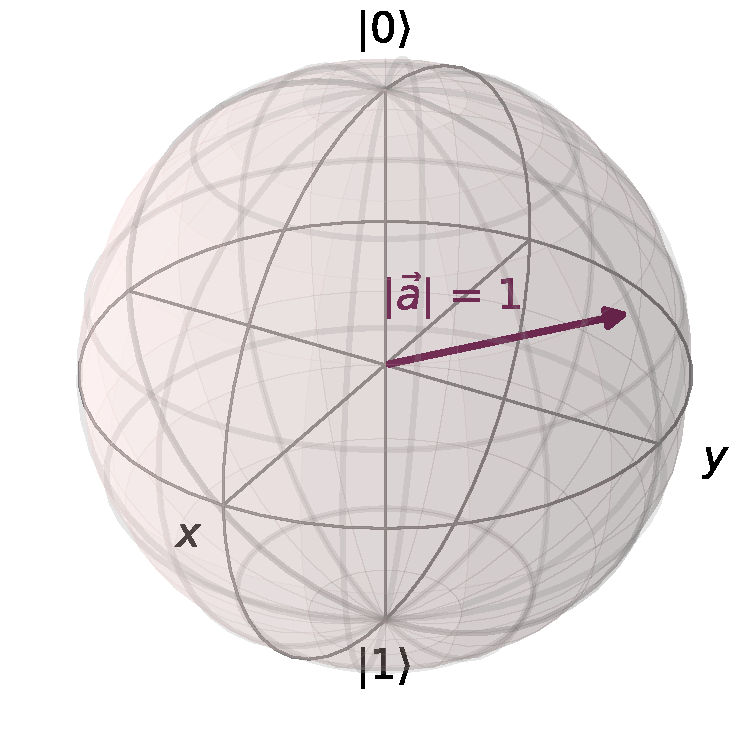
\includegraphics[]{Figs/Theory/bloch_sphere_pure.pdf}
    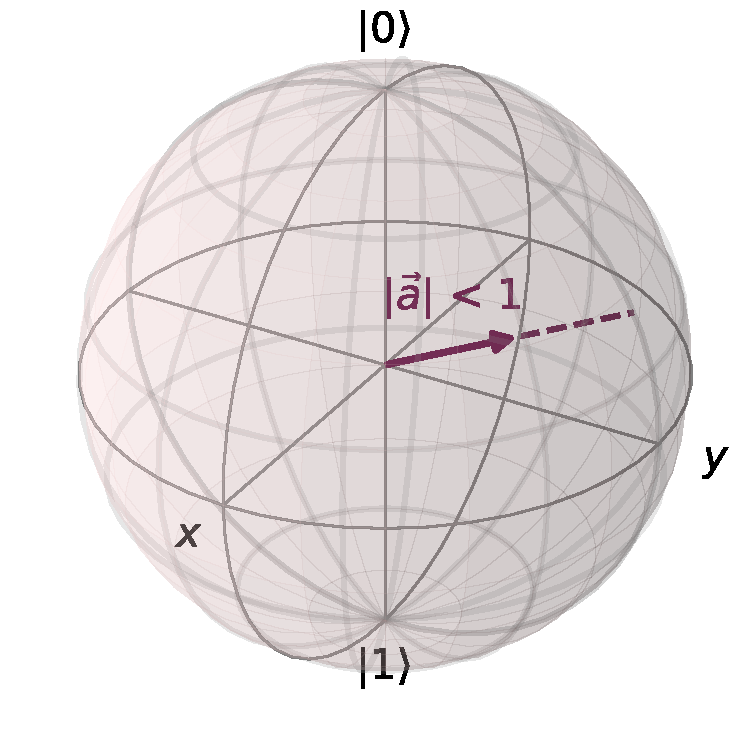
\includegraphics[]{Figs/Theory/bloch_sphere_mixed.pdf}
    \caption{Pure state (top) and mixed state (bottom) visualized on the Bloch Sphere.}
    \label{fig:bloch_sphere_density_matrix}
\end{marginfigure}

The representation in equation \ref{eq:density_of_qubit} provides even more flexibility. When we have a pure state, $|\Vec{a}| = 1$, and the vector points to the unit sphere. However $\rho = \frac12 \; \identity$ is also a valid density matrix, namely the fully mixed matrix. Here $|\Vec{a}|=0$. In terms of the Bloch sphere, we can think of pure states as living on the surface while mixed states will have an associated vector pointing somewhere inside $|\Vec{a}|<1\Leftrightarrow \Tr(\rho^2) < 1$.

\subsection{The Temperature of the System}
Even at low temperatures, one should expect to see the temperature have an effect on the qubit. If we consider the qubit connected to the environment as bath, we know from statistical physics that the probability of finding the qubit in different energy states is determined by Boltzmann statistics \cite{kittel_thermal_1980}. Limiting ourselves to a two level system, we would find the qubit in $\ket{0}$ with $\text{prob}(\ket{0}) = 1 / (1 + e^{-\beta\omega_{01}})$ and $\text{prob}(\ket{1}) = e^{-\beta\omega_{01}} / (1 + e^{-\beta\omega_{01}}).$ While the idea is to initialize the qubit in $\ket{0}$, this fact means that waiting until equilibrium our qubit would be in:
\begin{equation}\label{eq:equilibrium_qubit_density_matrix}
    \rho_{\text{equilibrium}} = \frac{1}{1 + e^{-\beta\omega_{01}}}\begin{pmatrix}
        1 & 0 \\
        0 & e^{-\beta\omega_{01}}
    \end{pmatrix}
\end{equation}

\subsection{Longitudinal Relaxation}\label{sec:theory_t1}
If the qubit exchanges energy with the environment it could drive transitions between the states $\ket{1} \leftrightarrow \ket{0}$. The relaxation from $\ket{0}\to\ket{1}$ at a rate $\Gamma_\downarrow$ will in the Lindblad equation be described by the Lindblad operator $L_{\downarrow} = \sqrt{\Gamma_{\downarrow}} \ket{0}\bra{1}$ and correspondingly $L{_\uparrow} = \sqrt{\Gamma_{\uparrow}} \ket{1}\bra{0}$ will describe the excitement. A qubit which relaxes energy into the environment will have time dynamics which follows\footnote{We use here the anti-commutator $\{A, B\} = AB + BA$ to write the Lindbladian a bit more compactly}: 
\begin{align*}
    \dot{\rho}(t) &= \mathcal{D}[L_{\downarrow}]\rho(t)) \\
    \dot{\rho}(t) &= \Gamma_\downarrow\left(\ket{0}\bra{1} \rho(t) \ket{1}\bra{0} - \frac12 \{\ket{1}\bra{0}\ket{0}\bra{1}, \rho(t)\}\right) \\
    \dot{\rho}(t) &= \Gamma_\downarrow\left(\rho_{11}\ket{0}\bra{0} - \rho_{11} \ket{1}\bra{1} - \frac12\left(\rho_{01}\ket{1}\bra{0} + \rho_{10}\ket{0}\bra{1}\right)\right)
\end{align*}
By looking at the individual components of the density matrix, we find:
\begin{align*}
    &\dot{\rho}_{00}(t) = \Gamma_\downarrow\rho_{11}(t)  &\dot{\rho}_{10}(t) = -\frac12\Gamma_\downarrow\rho_{10}(t)\; \\   
    &\dot{\rho}_{01}(t) = \frac12 \Gamma_\downarrow\rho_{01}(t)   &\dot{\rho}_{11}(t) = -\Gamma_\downarrow\rho_{11}(t)\;
\end{align*}
% \end{align*}
When adding the contribution from $\mathcal{D}[L_\uparrow]\rho(t)$ and introducing $\Gamma_1 = \Gamma_\downarrow + \Gamma_\uparrow$, we find the diagonal elements to:
\begin{equation}
    \dot{\rho}_{00}(t) = \Gamma_\downarrow\rho_{11}(t) - \Gamma_\uparrow\rho_{00}(t), \quad \dot{\rho}_{11}(t) = \Gamma_\uparrow\rho_{00}(t)-\Gamma_\downarrow\rho_{11}(t)\; \\   
\end{equation}
and the off-diagonal to:
\begin{equation}
    \dot{\rho}_{01}(t) = -\frac12 \Gamma_1\rho_{01}(t),  \quad \dot{\rho}_{10}(t) = -\frac12\Gamma_1\rho_{10}(t) \;
\end{equation}
The diagonal elements make up a set of coupled differential equation, solving for these two\footnote{This is done by writing the differential equation in matrix representation, by diagonalizing the coefficient we find a basis were the differential equation are decoupled. Solving here and transforming back gives the solution. }  and using $\Tr(\rho) = \rho_{00} + \rho_{11} = 1$ gives:
\begin{equation}
\rho_{00}(t) = \frac{\Gamma_\downarrow}{\Gamma_\uparrow + \Gamma_\downarrow} + \left(\rho_{00}(t=0) -  \frac{\Gamma_\downarrow}{\Gamma_\uparrow + \Gamma_\downarrow}\right)e^{-t(\Gamma_\uparrow + \Gamma_\downarrow)}
\end{equation}
and 
\begin{equation}    
\rho_{11}(t) = \frac{\Gamma_\uparrow}{\Gamma_\uparrow + \Gamma_\downarrow}+\left( \rho_{11}(t=0) -\frac{ \Gamma_\uparrow}{\Gamma_\uparrow + \Gamma_\downarrow}\right) e^{-t(\Gamma_\uparrow + \Gamma_\downarrow)}
\end{equation}
while the off-diagonals are simply solved by exponential decay:
\begin{equation}
    \rho_{01}(t) = e^{-\Gamma_1 t/2}\rho_{01}(t=0), \quad \rho_{10}(t) = e^{-\Gamma_1 t/2}\rho_{10}(t=0)
\end{equation}
From this we see the effects of energy exchange: excitations and relaxations effect the occupation of $\ket{0}$ and $\ket{1}$ until they are in an equilibrium. Further, the energy exchange also leads to decoherence on the diagonal with a rate of $\Gamma_1/2$. 
\begin{marginfigure}
    \centering
    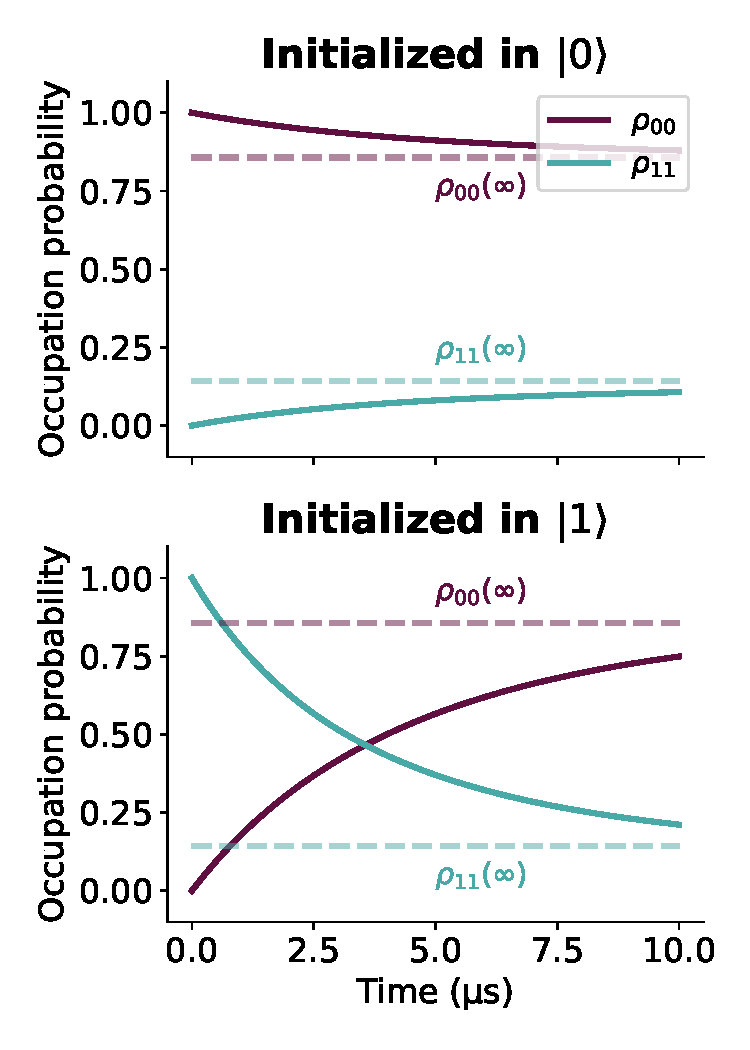
\includegraphics[]{Simulations/simulations_of_calibrations/Figs/qubit_T1_theroy.pdf}
    \caption{Evolution of the diagonal density elements if the qubit is initilzied in $\ket{0}$ or $\ket{1}$ respectively.}
    \label{fig:qubit_t1_theory}
\end{marginfigure}
We can also compare the equilibrium position $t\to\infty$ with the equilibrium state described by the Boltzmann statistics in equation \ref{eq:equilibrium_qubit_density_matrix}. Here we find that the rates should satisfy:
\begin{equation}
    \frac{\Gamma_\downarrow}{\Gamma_\uparrow + \Gamma_\downarrow} = \frac{1}{1 + e^{-\beta\omega_{01}}} \Rightarrow \frac{\Gamma_\uparrow}{\Gamma_\downarrow} =e^{-\beta\omega_{01}} 
\end{equation}
For low temperaturs $\beta \omega_{01} \ll 1$, this means that $\Gamma_1 \approx \Gamma_\downarrow$. The characteristic time of the decay from an arbitrary density matrix to the equilibrium is described by the characteristic time $T_1 = \frac{1}{\Gamma_1}$.

\subsection{Dephasing}\label{sec:theory_t2}
If the environment connect to the energy splitting and alters it and we will experience dephasing of the qubit. Mostly, dephasing is split into two parts: 

\textbf{A slow part} that compared to the experiment we run, such that we can consider it a constant shift of the qubit frequency $\omega \to \omega + \delta_\omega$. We can look at the consequences of this by simply evolving the equations unitarily. 

% \begin{marginfigure}
%     \centering
%     \missingfigure{Slow dephasing}
%     \missingfigure{Fast dephasing}
%     \caption{Caption}
%     \label{fig:enter-label}
% \end{marginfigure}

\textbf{A faster part} which changes multiple times during the experiment. If we consider this a normal distributed contribution to $\sigma_z$ at each small timestep, we can model this like the random unitary example, we considered in section \ref{sec:random_unitary_transformation} in which we would have the operator $L_\phi = \sqrt{\Gamma_\phi}\sigma_z$. If we apply this Lindblad operator, the time evolution would look like:
\begin{equation}
    \dot{\rho}(t) = \mathcal{D}[L_{\phi}]\rho(t)) = \Gamma_\phi\left(\sigma_z \rho(t) \sigma_z -\frac12( \sigma_z^2 \rho(t) + \rho(t) \sigma_z^2)\right)
\end{equation}
Since $\sigma_z^2 = \identity$ and $\sigma_z \rho(t) \sigma_z$ flips the sign of the diagonals, we get:
\begin{equation}
    \dot{\rho}(t) = - \Gamma_\phi \left(\ket{0}\bra{1}\rho_{01} - \ket{0}\bra{1}\rho_{01}\right)
\end{equation}
This gives us an extra contribution to the coherence terms, which are simply solved by:
\begin{equation}
    \rho_{01}(t) = e^{-\Gamma_\phi t}\rho_{01}(t=0), \quad \rho_{10}(t) = e^{-\Gamma_\phi t}\rho_{10}(t=0)
\end{equation}
So if were to combine the decays from this section and the last, the total dephasing rate would come out to be:
\begin{equation}
    \Gamma_2 = \Gamma_\phi + \frac12\Gamma_1 
\end{equation}
This is often described by the characteristic time of dephasing:
\begin{equation}\label{eq:t2_equation}
    T_2 = \frac{1}{\Gamma_2} = \frac{1}{\Gamma_\phi + \frac12\Gamma_1 } 
\end{equation}



% note:
% \begin{itemize}
%     \item This can probably be formulated better with the use of "Simple Derivation of the Lindblad Equation" where they introduce the random unitary operator to start phases change . Lindblad operator is $L = \sqrt{\Gamma_\phi}\sigma_z$
%     \item Maybe we can extract this from writing out the random unitary with the $\sigma_z$
% \end{itemize}

% If qubits instead connect longitudinally (along the $z-axis$) they can alter the qubit frequency $\omega_{01}$ which setts us at a disadvantage. Since we normally think about the $x-$ and $y-$axis in the rotating frame with the frequency $\omega_{01}$ any changes to the qubit frequency would speed up / slow down the actual rotation, and ultimately we lose information about the actual phase of the qubit. 

% Since there is no energy exchange with the environment this is a unitary process, and it is theory possible to reverse the effect and place the qubit back in the reference frame we know. However, this would assume that we have complete information about the time-dependence of the effective qubit frequency which is not realistic. With a clever use of gates, we can however decouple the pulse by using dynamical decoupling schemes which we will shortly return to in the section about calibrating the characteristic dephasing time $T_2$. *The concept is simply to apply $X_{\pi}$ pulses frequently to refocus the noise. Thus if some qubit initializations precess faster or slower adding a $X_\pi$ gate would flip the order allowing the fast ones to cast up and the slow ones to fall back to the actual qubit frequency

% The rate of dephasing has two components, one from the stochastic "pure" dephasing time described above. This rate is given as $\Gamma_\phi$. The second contribution comes from energy relaxation since any superposition would lose all phase information once collapsed. Think of the $\frac{1}{\sqrt(2)}\left(\ket{0} + e^{i\phi}\ket{1}\right)$ superposition. If $\ket{1}$ were to decay to $\ket{0}$ the phase of the qubit state would also be lost. The total dephasing rate can be found by:
% $$\Gamma_{2}=\Gamma_\phi+\frac{\Gamma_{1}}{2}$$
% and the characteristic dephasing time is given by:
% $$T_2=\frac{1}{\Gamma_{2}}$$

\subsection{Resonator Decays}\label{sec:resonator_decays}
The coupled resonator also leaks photon to the environment. This happens with a much higher rate since it is directly coupled to the feed line. The output of photon also consist of two parts, unwanted dissipation to the environment and leakage to the feed line which we are able to detect. For photon loss the Lindbladian operator is given by $L = \sqrt{\kappa}a$, where kappa is the rate of dissipation.

In section \ref{sec:driving_resonator_iq_plane}, we found a differential equation for the pointer state of a coherent state, when we drive the resonator. If we also consider the Lindbladian term, we get a further addition to the time dependence of $a$ in the Heisenberg picture since it takes the form of $\frac{d}{dt}a(t) = i[H_eff, a(t)] +  \mathcal{D}[\sqrt{\kappa}a](a)$\footnote{While we only discussed the equations of motion the Heisenberg picture operators take almost exactly the same form. However, it changes the sign of the commutator. One could check this by writing out the expectation values.}. Here $\mathcal{D}[\sqrt{\kappa}a](a)$ is given by:
\begin{equation}
    \mathcal{D}[\sqrt{\kappa}a](a) = \kappa \left(a^\dagger a a -\frac12 \left(a^\dagger a a + a a^\dagger a \right) \right)
\end{equation}
Using the commutator relation $\comm{a}{a^\dagger} = 1$, this can be reduced to
\begin{equation}
    \mathcal{D}[\sqrt{\kappa}a](a) = -\frac{1}{2}\kappa a 
\end{equation}
If we reintroduced this into the equations of motion, we find an additional term in the differential equation for the pointer states:
\begin{equation}\label{eq:resonator_movement}
    \frac{d}{dt}\alpha(t) = - i \left(\omega_r - \omega_d \pm \chi\right) \alpha(t) + i\epsilon - \frac{\kappa}{2}\alpha(t) 
\end{equation}
This dissipative term takes the effect of pushing the coherent state closer to the origin. If we were to repeat the driving of the resonator with the dissipation, we see that driving off resonance gives a spiral instead of circle towards some steady state. These steady state values can also be found by solving for the steady state equation with $\dot{\alpha}(t) = 0$. We find:
\begin{equation}
    \alpha_{\text{ss}} = \frac{-\epsilon}{(\omega_r - \omega_d \pm \chi) - i \kappa / 2}
\end{equation}
From which we can extract the steady state amplitude from equation \ref{eq:steady_state_amplitude}:
\begin{equation}\label{eq:steady_state_amplitude}
    |\alpha_{\text{ss}}| = \frac{\epsilon}{\sqrt{(\omega_r - \omega_d \pm \chi)^2 + \kappa^2 / 4}}
\end{equation}
An example of driving the resonator with dissipation can be seen in figure \ref{fig:iq_movement_with_kappa}.

\begin{figure}
    \centering
    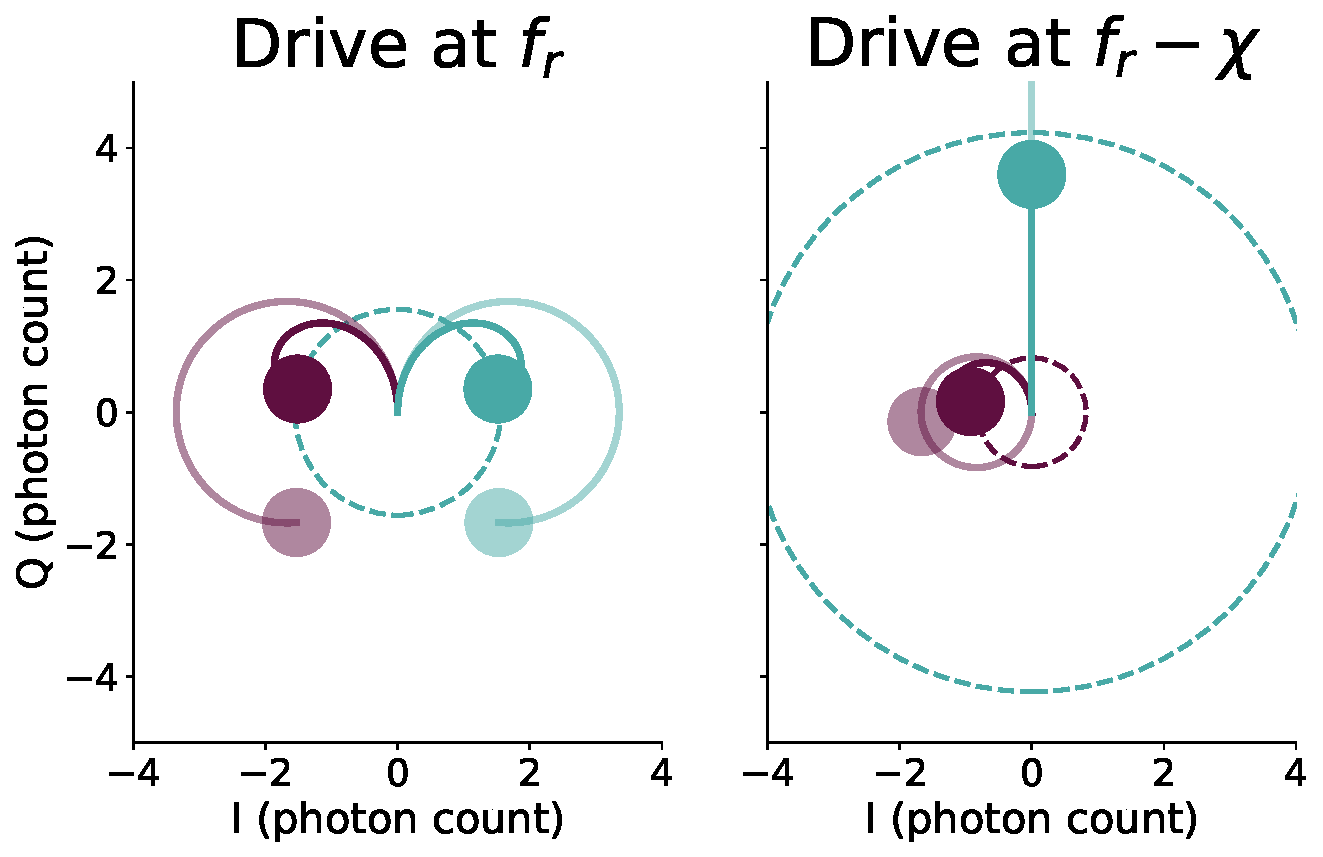
\includegraphics{Simulations/readout_simulations/IQ_movement_with_kappa.pdf}
    \caption{Driving of the resonator with the qubit in ground and excited state. The trajectories of the pointer states are shown together with the steady state amplitude.}
    \label{fig:iq_movement_with_kappa}
\end{figure}

% One could follow the same calculations and arguments as with the qubit $T_1$ and would find the Lindblad operator $\sqrt{\kappa}a$. Ultimately this also gives a decay of resonator towards its equlibrium which we can assume to be ground state if it is cold enough. The rate $\kappa$ described the rate at which photons escape the resonator.

